\documentclass[12pt]{article}

% Include necessary packages
\usepackage[utf8]{inputenc} % Support for utf8 encoding
\usepackage[T1]{fontenc}    % Support for more font encoding
\usepackage{graphicx}       % To include images
\usepackage[hidelinks]{hyperref}       
\usepackage{amsmath}        % For mathematical formulas
\usepackage{geometry}       % For page layout
\usepackage{xcolor}
\usepackage{CJKutf8}
\geometry{a4paper,scale=0.8} % A4 paper, 80% page utilization

% Begin document
\begin{document}

% Title page
\begin{titlepage}
    \newcommand{\HRule}{\rule{\linewidth}{0.5mm}}
    \centering
    \vspace*{60px}

    \HRule \\[0.4cm]
    { \huge \bfseries BGP Fast Failure Detection using BFD}
    \HRule \\[0.4cm]

    \vspace*{30px}
    {\Large\bfseries INF645 Independent Project Report\par}
    \vspace{30px}
    {\Large\itshape Chuhao Tang\par}
    \vspace{30px}
    Major \& Class: \textit{M2 Internet of Things}\par
    \vfill
    {\large \today\par}
\end{titlepage}

% Table of contents
\tableofcontents
\newpage

% Section 1
\section{Introduction}
\subsection{Reason for choosing this topic}
Last year's internship at Cisco Meraki taught me a lot about the IPSec related network knowledge in VPP. Its high performance and scalability in handling network packets made me
interested in the platform and networking stuff, so I want to continue to learn more about networking and routing rules.

This year's internship continue with the CNHE team at Cisco Meraki. The team manager gave
me a lot of pre-work so that I could get up to speed when I start my internship. So much of the independent project is based on the requirements given to me by the manager, which are, knowing latest methods and protocols used for fast failure detection for BGP routing (for example BFD) and how others perform BGP failure/fast failure detection

For my future career plan, I am looking to continue to work as a network engineer or in a
network security related direction. So I think it's important to understand and deploy the BGP
protocol. Both network engineers and network security can not do without the processing of BGP
packets. I hope that this independent project will help me to have a deeper understanding of
networking so that I can find a great job after graduation.

\subsection{Border Gateway Protocol (BGP)}
The Border Gateway Protocol (BGP) is the cornerstone of the internet's global routing system \cite{ref12}, enabling data packets to find their way across the complex maze of interconnected networks that make up the internet. As a path vector protocol, BGP is responsible for making decisions about routing based on paths, network policies, or rule-sets configured by network administrators\cite{ref6}, which allows it to manage how packets are routed between autonomous systems (ASes). The ASes are the large collections of IP networks managed by single entities or organizations.

BGP plays a crucial role in the functionality and performance of the internet. It allows networks to automatically provide and receive routing information with other networks, facilitating the dynamic, automated routing of data. Moreover, BGP is instrumental in the implementation of  routing policies, which allows ASes to control the flow of traffic based on various criteria, including traffic origin, destination, and path characteristics.

However, despite its crucial role, BGP also faces significant challenges related to fast failure detection and recovery. The protocol's mechanism for detecting network failures and rerouting traffic is using KEEPALIVE packets, which often resulting in prolonged downtime before connectivity is restored. With a default hold time of 180 seconds on a Cisco router, BGP KEEPALIVE packets are sent every 60 seconds\cite{ref3}. This delay is primarily due to the time-intensive process of BGP route withdrawals and the propagation of these changes through the network. Additionally, the lack of an efficient and standardized method for immediate failure detection within BGP further exacerbates the problem, leaving networks vulnerable to transient failures and unstable paths.

\subsection{Bidirectional Forwarding Detection (BFD)}
Bidirectional Forwarding Detection (BFD) is a detection protocol designed to provide fast forwarding path
failure detection times for all media types, encapsulations, topologies, and routing protocols.\cite{ref1}

To address the limitations of BGP, the integration of BFD with BGP has been proposed and increasingly implemented. BFD offers a rapid failure detection mechanism, capable of identifying link failures within milliseconds, significantly improving the resilience and responsiveness of network infrastructures. However, deploying BFD alongside BGP introduces its own set of challenges, including the increased overhead on networking equipment, the need for careful tuning to avoid false positives, and the complexity of managing BFD sessions across diverse and large network environments. Despite these consideration, the combined use of BFD for fast failure detection with BGP's powerful routing capabilities represents a vital advancement towards achieving more reliable and dynamic network operations.

BFD sessions usually have three states, which are shown in the following context. DOWN: The session at this end has been closed or just created. The DOWN state indicates that the forwarding path is unavailable and the upper layer application linked to the BFD session needs to take appropriate measures, such as primary and backup path switching. INIT: This end can already communicate with the other end, and this end wants the session to enter UP state. UP: The local session has been successfully established. The UP state indicates that the forwarding path is available. The state machine migration mechanism is shown in Figure \ref{fig:example}.

\begin{figure}[h]
    \centering
    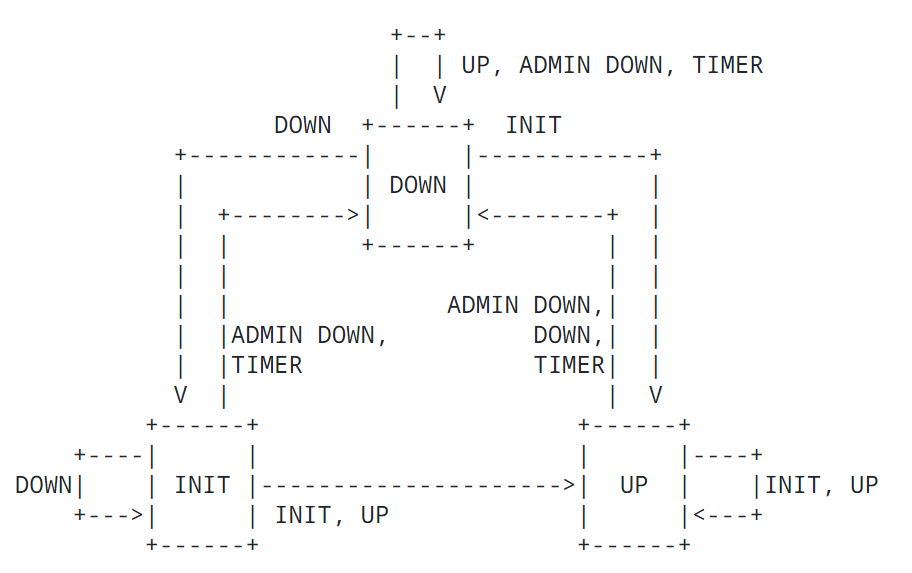
\includegraphics[width=0.5\textwidth]{Graph/BFD state machine.png}
    \caption{BFD state machine \cite{ref4}} 
    \label{fig:example} 
    
\end{figure}


\subsection{Graphical Network Simulator-3(GNS3)}
GNS3, or Graphical Network Simulator-3, is a highly regarded network software emulator first introduced in 2008\cite{ref5}. It provides a flexible and intuitive platform for network professionals worldwide, enabling them to emulate, configure, test, and troubleshoot both virtual and real network environments. This tool stands out by allowing the combination of virtual and real devices, facilitating the simulation of complex networks which can range from simple designs running on a laptop to extensive architectures hosted across multiple servers or even in the cloud.

A key feature of GNS3 is the simulation of the Cisco IOS using dynamips emulation software, which provides hands-on experience in simulating the workings of real network hardware. This feature is invaluable for those who need to test network configurations before deployment, and GNS3 supports a wide range of network devices from different vendors, providing a versatile environment for learning and testing network concepts and configurations.

\newpage
% Section 2
\section{Related research work on BGP fast failure detection}
\subsection{BGP retransmission combined with BFD}
For regular BGP protocols, the routing decisions are efficient. But when talking about their convergence time, i.e., the time it takes to recognize and react to changes in the network, can be slow, thus affecting network performance and reliability. The main reason for slow convergence is BGP's reliance on periodic updates and the time it takes to detect a failed link before initiating a route change. To reduce these delays and improve link failure detection, BGP can be combined with BFD, a faster and more efficient protocol designed to quickly detect failures in paths between neighboring forwarding engines.

BFD operates independently of media, data link protocols, and routing protocols, providing a low overhead, short duration method for detecting faults on paths between two forwarding planes. When integrated with BGP, BFD can be used as a fast fault detection mechanism that greatly reduces convergence time by immediately notifying BGP of any link failures.The BGP fast reroute and BFD linkage technique can well meet this requirement \cite{ref7}, as shown in Figure \ref{fig:BGP fast reroute combined with BFD}, by calculating the alternate path in advance, quickly detecting primary path failures, and directly, without relying on the convergence of the control plane, in the event of a primary path failure switch to the alternate path in the forwarding plane without relying on the convergence of the control plane in case of primary path failure, which greatly shortens the service disruption time.

\begin{figure}[h]
    \centering
    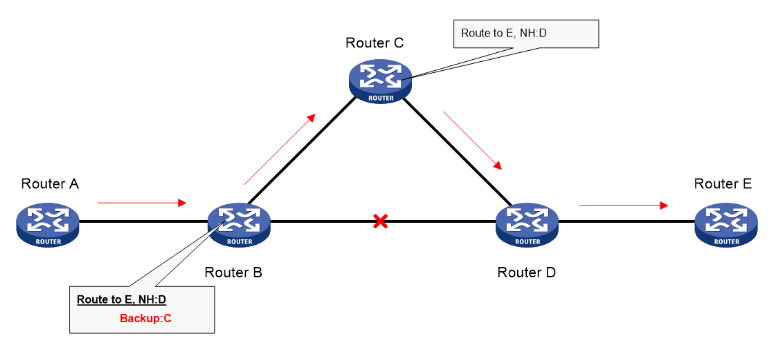
\includegraphics[width=0.7\textwidth]{Graph/BGP fast reroute and BFD.png}
    \caption{BGP fast reroute combined with BFD \cite{ref7}} 
    \label{fig:BGP fast reroute combined with BFD} 
    
\end{figure}

By utilizing BFD's rapid fault detection capabilities, network operators can significantly improve BGP's responsiveness in dynamic environments where network reliability and uptime are critical. This synergy not only optimizes routing decisions and reduces packet loss, but also supports the demands of modern high-speed Internet applications where even minor delays can impact the user experience.The combination of BGP retransmission and BFD represents a strategic approach to overcoming the inherent limitations of traditional routing protocols, and marks a significant step forward in the evolution of network management and operational efficiency.

\subsection{Multithread recovery algorithm in BGP}
The adoption of a multi-threaded approach to a complex BGP-based fault recovery system represents a major advancement in network recovery capability and efficiency. By separating the fault recovery process into dedicated threads that run concurrently with multiple BGP session threads, the system ensures that the fault detection and recovery process is both fast and efficient. The design leverages the capabilities of the BFD protocol to quickly identify link failures, a key feature for maintaining uninterrupted network service and minimizing the impact on data flow.

Dynamic route generation algorithms play a key role in this architecture. Once a failure is detected, the algorithm is triggered to compute alternative paths, effectively rerouting traffic and ensuring that packets reach their destinations with minimal delay. This proactive approach not only maintains the integrity of data transmission, but also prevents the exacerbation of BGP loops-frequent updates due to routing instability can increase network traffic and potential instability.

Simulation studies emphasize the effectiveness of this multithreaded approach. By comparing scenarios with and without this enhanced fault recovery system. The algorithm is also implemented using Thread BGP (TBGP) \cite{ref8}, a concept that employs multithreading techniques in BGP implementations with the aim of improving the efficiency and processing speed of routing computations, especially in large-scale or high-performance network environments. Also the Failure proportion based article gives support for experimental simulations as shown in Figure \ref{fig:Test result of TBGP}.

\begin{figure}[h]
    \centering
    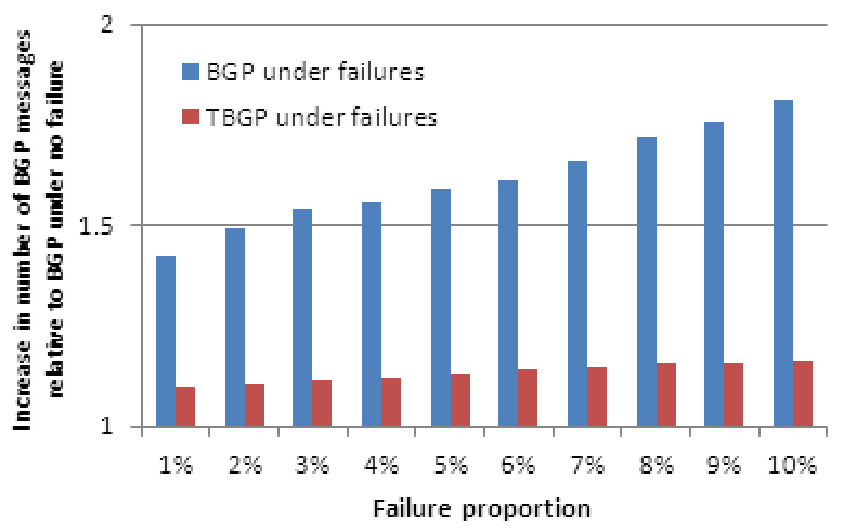
\includegraphics[width=0.7\textwidth]{Graph/TBGP.png}
    \caption{Test result of TBGP \cite{ref9}} 
    \label{fig:Test result of TBGP} 
    
\end{figure}

In summary, integrating multiple threads to handle BGP-based fault recovery, utilizing BFD for fast fault detection, and employing dynamic route generation algorithms provides a powerful solution to network reliability and efficiency challenges. The dramatic reduction in packet loss duration and BGP message overload highlights the potential of this approach to significantly improve the resilience and operational capabilities of modern networks.


\subsection{Seamless Bidirectional Forwarding Detection (SBFD)}
Seamless BFD (SBFD) is an enhanced implementation of the BFD protocol designed to simplify and speed up the process of establishing a bi-directional forwarding detection mechanism between any two network nodes \cite{ref10}. BFD is an underlying, fast mechanism for detecting failures in the link between two connected devices in a network.SBFD builds on this foundation by adding new features and optimizations that simplify the state machine of BFD ( SBFD supports only UP and DOWN states), shortens the session negotiation time, and its detection speed is faster than BFD.SBFD is suitable for situations where only one end needs to perform link state detection.

In an SBFD session, the roles of the device are categorized into Initiator and Reflector, which is shown in the Figure \ref{fig:Functionality of SBFD}. The network shown in Figure 7 as an example, Router A as the Initiator sends SBFD control messages to Router E as the Reflector through the MPLS TE tunnel established based on SR (Segment Routing), as long as Router A is able to receive the SBFD control messages sent by Router E, the SRLSP path from Router A to Router E is considered reachable. Router A considers the SRLSP path from Router A to Router E to be reachable as long as it can receive the SBFD control message from Router E.

\begin{figure}[h]
    \centering
    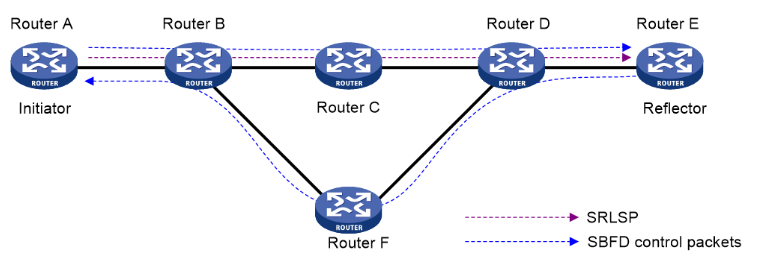
\includegraphics[width=0.7\textwidth]{Graph/SBFD.png}
    \caption{Functionality of SBFD \cite{ref7}} 
    \label{fig:Functionality of SBFD} 
    
\end{figure}

SBFD is particularly well suited for dynamic or large-scale network environments where rapid fault detection and recovery is critical to maintaining network stability and performance \cite{ref11}. For example, in data centers, large enterprise networks, or service provider networks, SBFD can improve network reliability and availability while reducing the configuration burden on network administrators.The introduction of SBFD represents a continuing advancement in network technology in the quest for greater efficiency and a better network user experience.

\newpage
% Section 3
\section{BGP implementation between ASes with different IGP protocols}
\subsection{General idea}
Building upon the foundational insights gained from previous research into the BGP fast retransmission and failure detection algorithm, I've acquired a profound understanding of the theoretical basis. However, for network engineers, only having theoretical knowledge is hard to follow the comprehensive expertise required to the complexities of real-world networking scenarios. The practical application of theoretical principles is crucial. It is with this realization that my research has shifted to a more applied phase.

This chapter are dedicated to building and analyzing a robust network infrastructure that can facilitate communication between different autonomous systems by implementing BGP. This platform is not a monolithic one, but consists of different Interior Gateway Protocols (IGPs) such as (Open Shortest-Path First)OSPF and (Routing Information Protocol)RIP, each of which operates in its own autonomous system. This configuration provides a unique opportunity to delve into the operational nuances and message exchange mechanisms between IGP and BGP. My research will mainly focus on the two protocols, OSPF and BGP.

First I will examine the different characteristics and behaviors of the IGP and BGP protocols in terms of information exchange and updating. Second, within this framework, I will explore the need for the deployment of BGP fast fault detection. The need for such a mechanism stems from the urgent need to maintain network stability and reliability in the face of link or node failures.Rapid fault detection in BGP is not just a theoretical construct, but an important operational requirement to ensure the resilience and efficiency of network communications.


\subsection{Implementation}
The basic configuration is shown as follows: the system consists of four routers and two PCs, with AR1, AR2 and APC in AS100 and BR1, BR2 and BPC in AS200. Figure \ref{fig:Implementation of BGP between ASes with different IGP protocols} shows the real implementation of the whole framework. 

\begin{figure}[h]
    \centering
    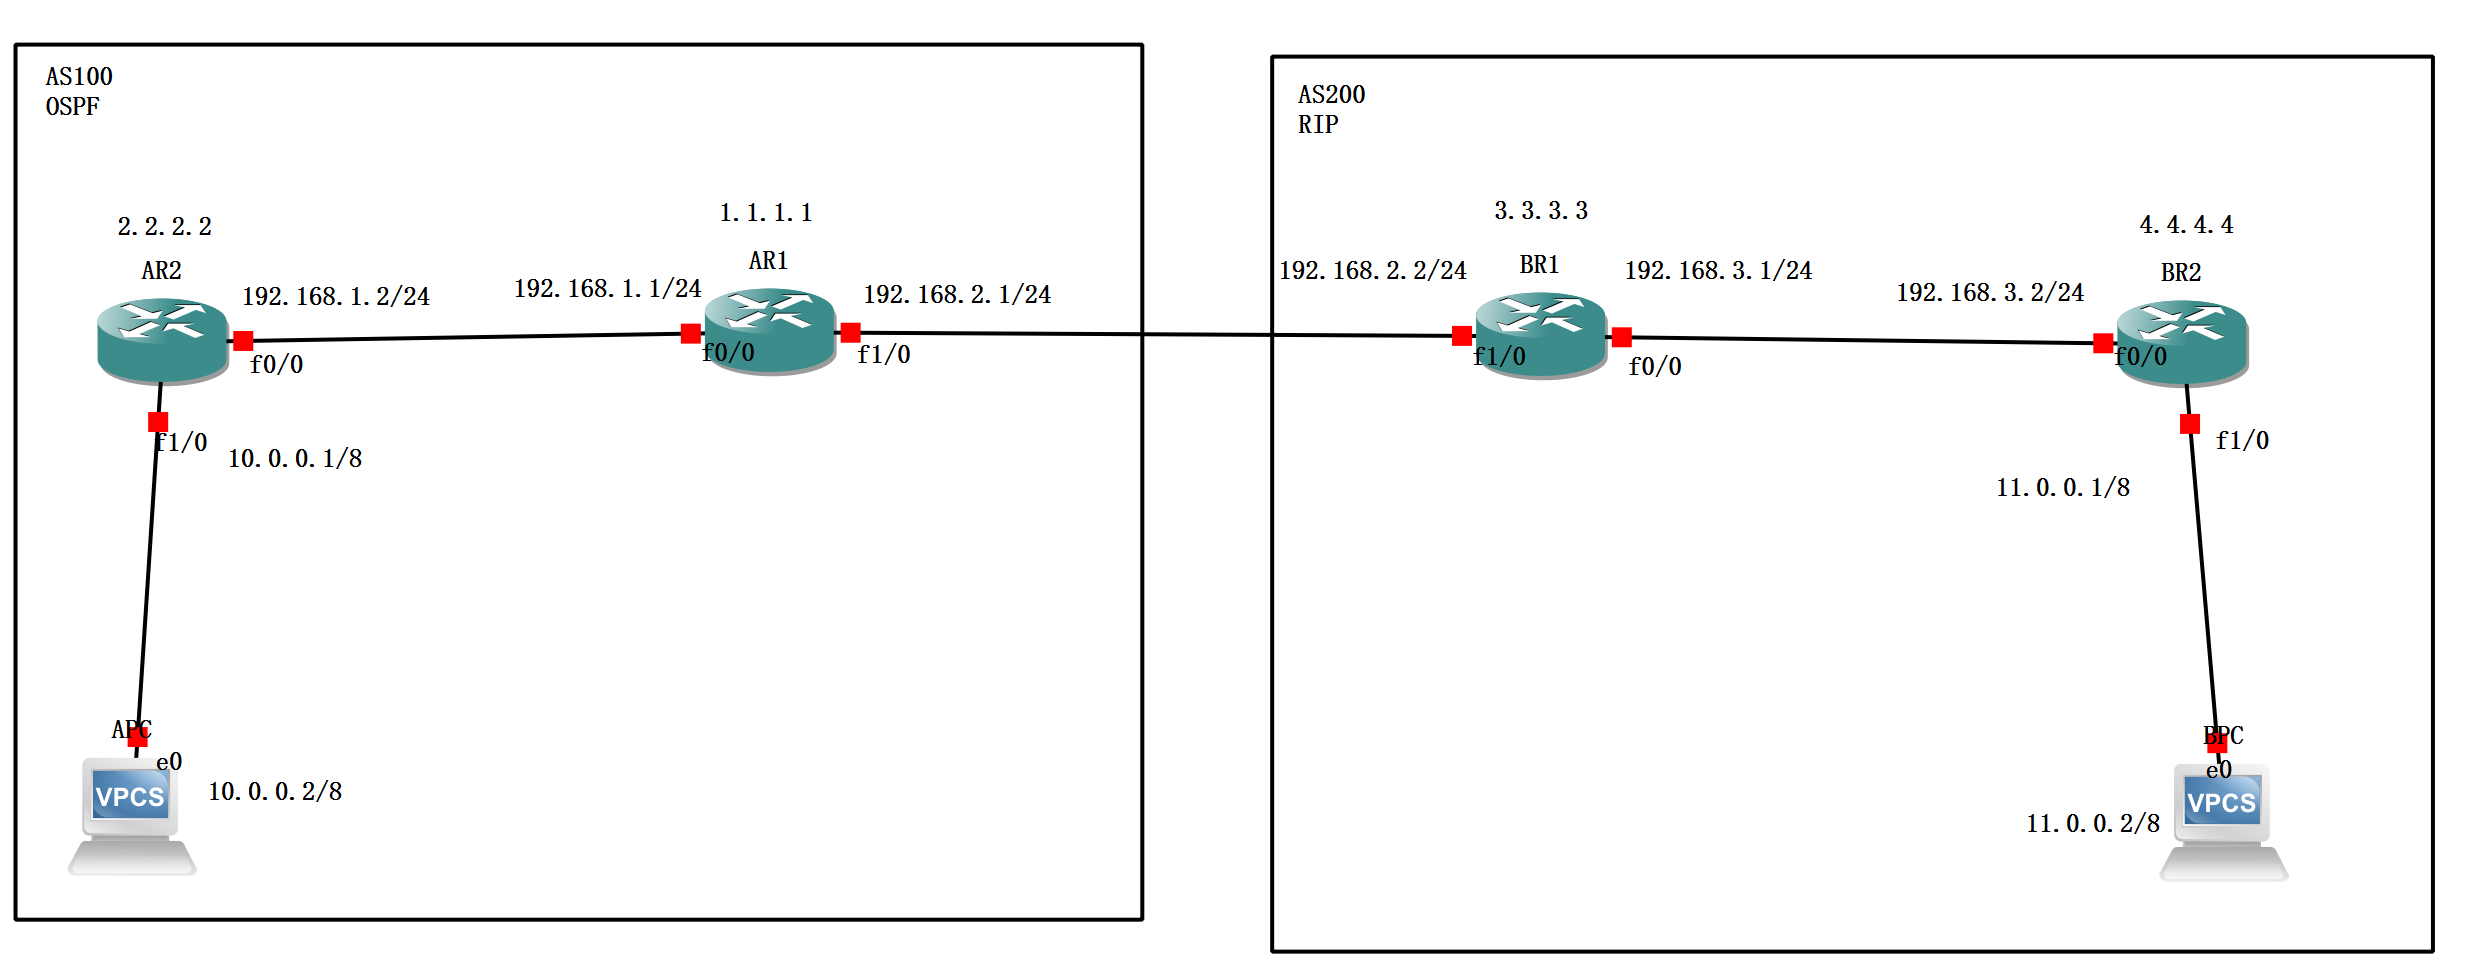
\includegraphics[width=0.9\textwidth,keepaspectratio]{Graph/BGP in different ASes.png}
    \caption{Implementation of BGP between ASes with different IGP protocols} 
    \label{fig:Implementation of BGP between ASes with different IGP protocols} 
\end{figure}

The two routers in AS100 use the OSPF protocol to exchange routing information in the 192.168.1.0/24 network segment, AR2 is directly connected to APC, and AR1 acts as a border router to the external router BR1. The two routers in AS200 use the RIP protocol to exchange routing information in the 192.168.3.0/24 network segment, and the routers in BR1 and BR2 use the RIP protocol to exchange routing information in the 192.168.3.0/24 network segment. connections are similar to those in AS100.

The direct connection between AR1 and BR1 uses the BGP protocol as a means of exchanging routing information between the two AS systems and serves as the only pathway between the two ASes. On this path, I will deploy the BFD protocol in order to observe the difference between traditional BGP retransmission and BGP retransmission with BFD deployed.

Since the configuration and the details of the router will not be illustrated, I chose the AR2 router ip route table and AR1 and BR1 between the path of the listening information to show the entire network connectivity. 

AR2 routing table as shown in the Figure \ref{fig:AR2 IP route table}, you can see that the formation of its routing table based on the local (L), directly connected to the port (C), the OSPF protocol (O) and the BGP protocol (B). This routing table shows all the topologies in AS100, which is the core characteristic of OSPF protocol, and also the segment information of remote host 11.0.0.2 through BGP.

\begin{figure}[h]
    \centering
    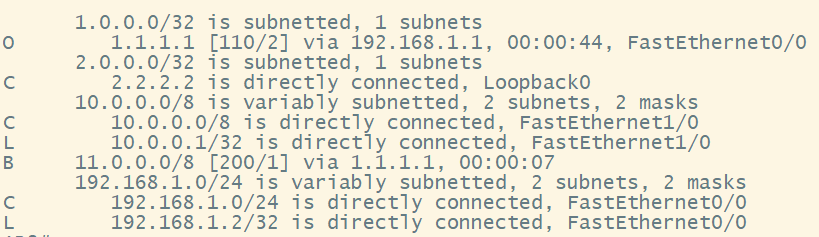
\includegraphics[width=0.75\textwidth,keepaspectratio]{Graph/AR2 ip route.png}
    \caption{AR2 IP route table} 
    \label{fig:AR2 IP route table} 
\end{figure}

The BGP protocol can be analyzed by using wireshark to observe the connection between AR1 and BR1, which is the network segment 192.168.2.0/24. As shown in the Figure \ref{fig:BGP packets}, you can observe the creation of the BGP protocol from scratch.The OPEN message indicates the establishment of the BGP peer KEEPALIVE message indicates the maintenance of the BGP connection, and the UPDATE message indicates the update of the BGP message.

\begin{figure}[h]
    \centering
    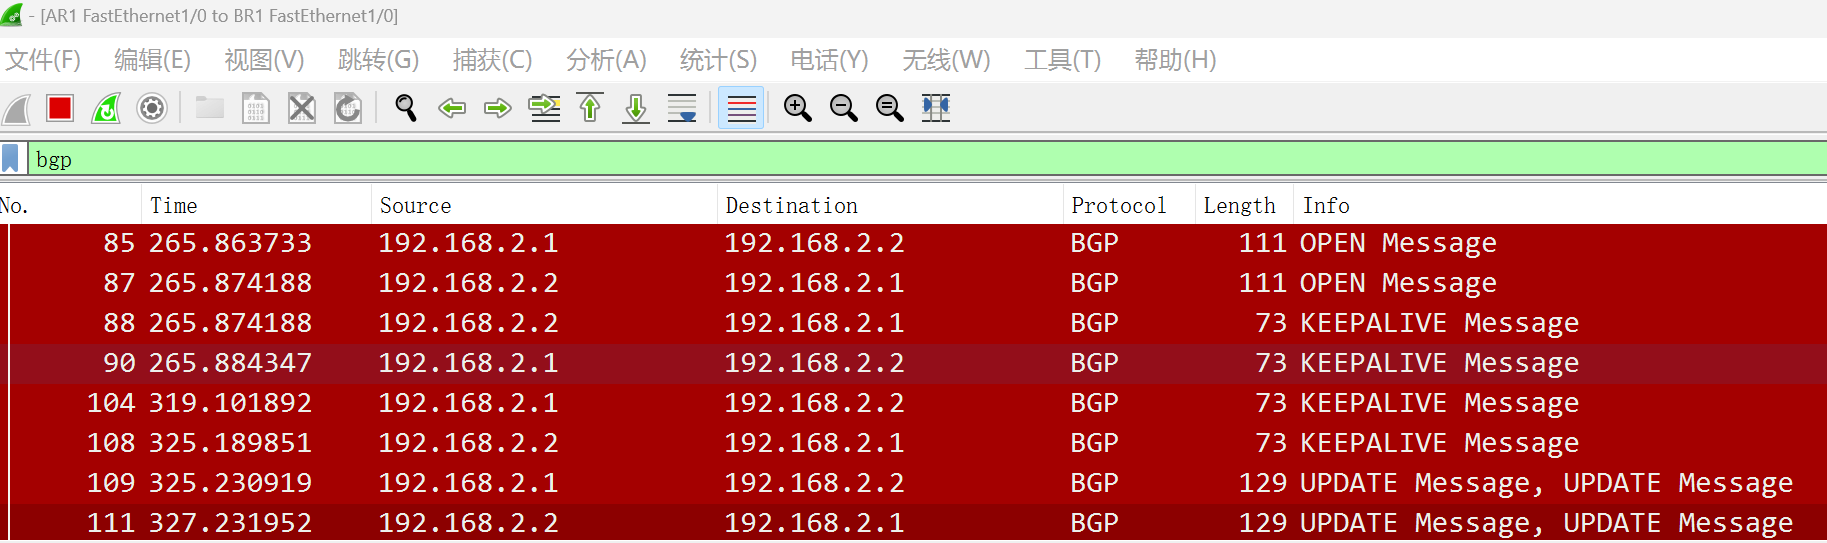
\includegraphics[width=0.7\textwidth,keepaspectratio]{Graph/BGP packets.png}
    \caption{BGP packets} 
    \label{fig:BGP packets} 
\end{figure}

In order to verify the connectivity of the entire network, I chose to ping the remote host BPC11.0.0.2 directly from APC10.0.0.2, so that I could verify the connectivity of the respective IGP protocols in the two ASes as well as the BGP protocols between the two ASes at the same time. The result is shown in the Figure \ref{fig:Ping message from APC to BPC}, and it can be seen that the implementation of the whole network is intact.

\begin{figure}[h]
    \centering
    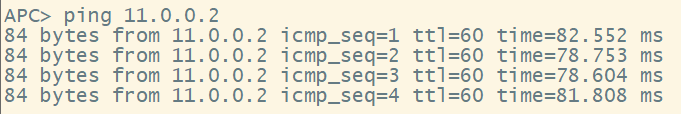
\includegraphics[width=0.8\textwidth,keepaspectratio]{Graph/ping msg.png}
    \caption{Ping message from APC to BPC} 
    \label{fig:Ping message from APC to BPC} 
\end{figure}


\subsection{Test and result}
The test environment and tools are shown below: GNS3, Cisco router image c7200, wireshark packet grabber tool and SecureCRT terminal emulation software.The main purpose of this test is to compare the difference in failure detection time between a BGP connection with BFD deployed and a BGP connection without BFD deployed, after a shutdown on one side or lose connection in the whole link.

The test I did is implementing BGP without BFD configured. I shutdown interface f1/0 of BR1 to simulate the disconnection of the connection. which will result in the result as Figure \ref{fig:BGP notification messages}. 

\begin{figure}[h]
    \centering
    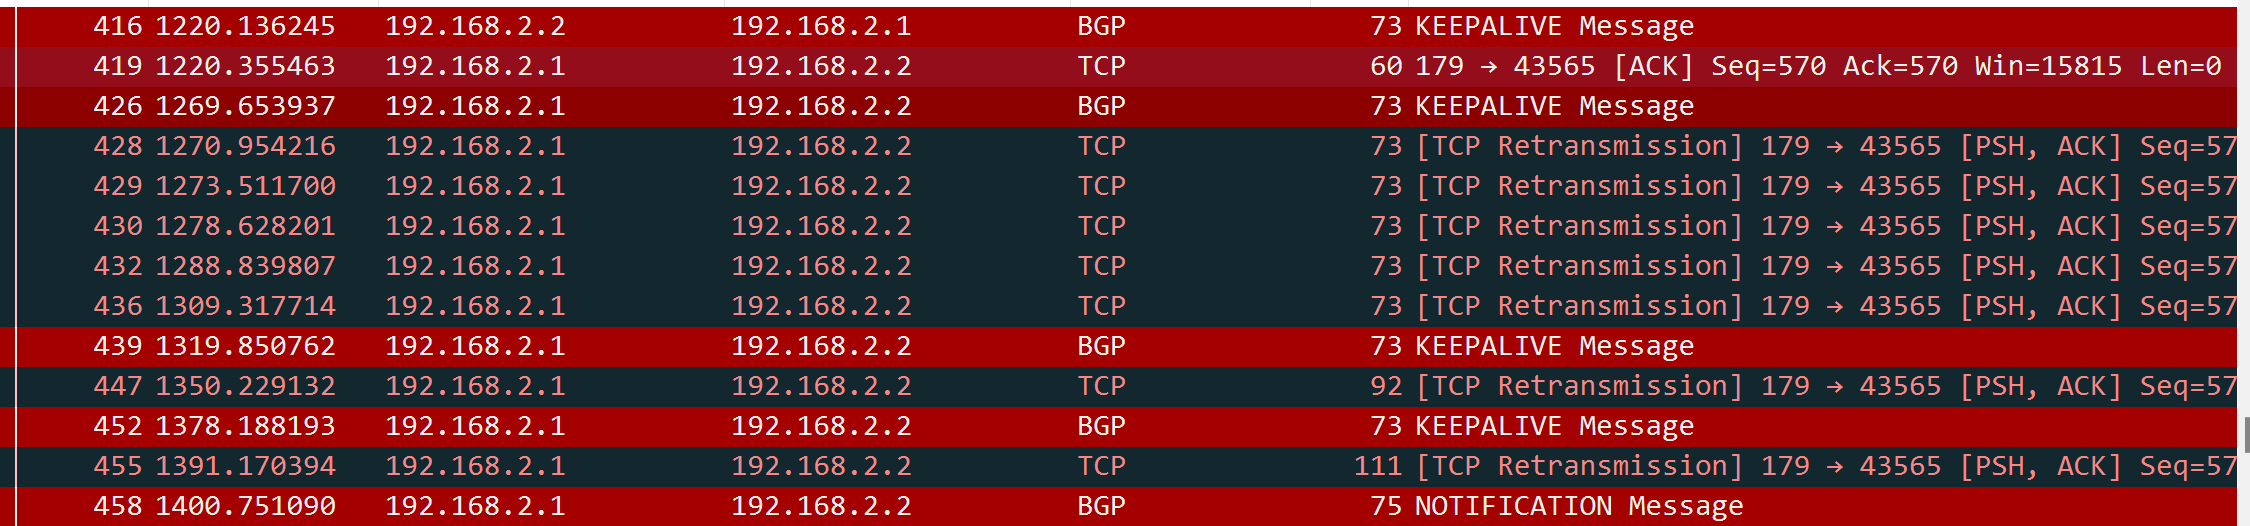
\includegraphics[width=0.85\textwidth,keepaspectratio]{Graph/BGP notification msg.png}
    \caption{BGP notification messages} 
    \label{fig:BGP notification messages} 
\end{figure}

The last time BR1 sends a KEEPALIVEBGP message can be considered as the point in time when it was just shutdown. When BR1 disconnects, AR1 keeps sending TCP reconnect requests to try to maintain the BGP connection. It is only after three KEEPALIVE BGP messages have been sent that AR1 sends a NOTIFICATION message as a way of announcing that BR2 is offline. It is easy to see that the time interval is \textit{$1400-1200 = 200$} seconds, which is about three and a half minutes. Such a long failure detection is undoubtedly very inefficient, even if there are only two AS systems and two border routers need three and a half minutes to detect the BGP connection disconnection, then a larger BGP network once one of the routers is down, then the entire network of BGP messages will become very slow to update.

Therefore, when I implementing BGP, I started BFD listening on the connection between AR1 and BR1 with the main configuration parameter \textcolor{blue}{\textit{bfd interval 500 min\_rx 500 multiplier 3}}, and the test result is shown as Figure \ref{fig:BFD failure detection}.

\begin{figure}[h]
    \centering
    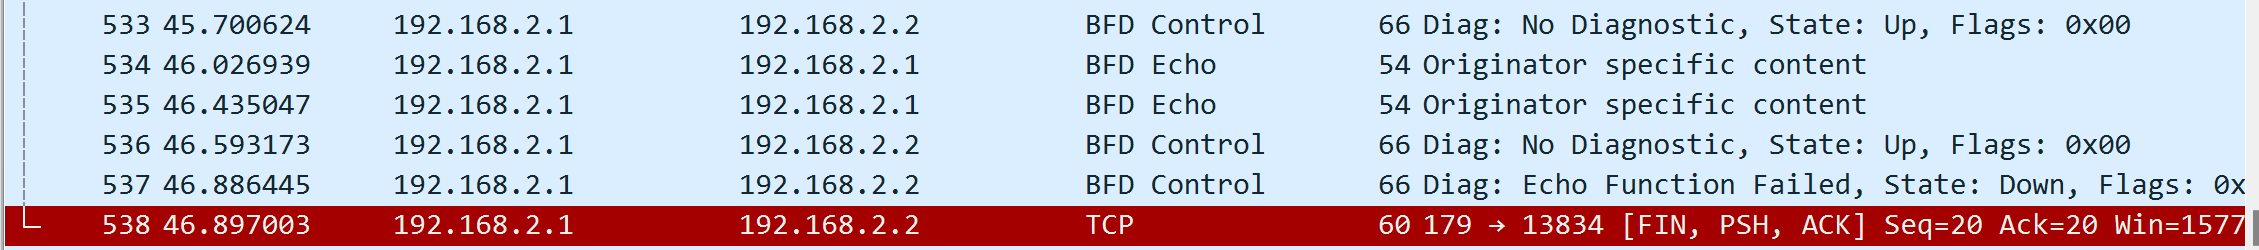
\includegraphics[width=1\textwidth,keepaspectratio]{Graph/BFD detection.png}
    \caption{BFD failure detection} 
    \label{fig:BFD failure detection} 
\end{figure}

When I configured BFD, setting multiplier to 3 means that as soon as when the BFD control packet sent by AR1 3 times is not sent back, it triggers TCP to end the FIN packet, that is, to disconnect the BGP connection, and after that, it declares BR1 unreachable within AS100 via OSPF protocol. Observing the packets through Wireshark, we can get that it only took \textit{$46.9-45.7=1.2$} seconds from the time BR2 went down to the time AR1 announced that it was disconnecting from TCP, which is more than 160 times faster than BGP without deploying BFD. In fact, by adjusting the interval and min rx in the BFD configuration, we can achieve faster BGP failure detection, which greatly improves the efficiency and enables us to react faster when we encounter router downtime in reality.

\newpage
% Section 4
\section{Platform building based on BFD link detection in BGP}
\subsection{General idea}
In the previous section, I used BGP messages to deliver routes in two AS systems using different IGP protocols. I also focused at a simple application of BFD over BGP and tested the performance gains from using BFD with a single path of BGP messages.

In this sections, I dive into the complex process of using BGP messages to facilitate the exchange of routing information between two ASes that use different IGP. This exploration includes a thorough examination of the direct deployment of BFD within the BGP framework, as well as an empirical evaluation of the performance enhancements resulting from the integration of BFD into the BGP message transmission path. Building on this foundational work, this chapter aims to construct and analyze a broader network infrastructure that includes multiple AS configurations. In order to optimize computational resources and minimize CPU overhead, the design strategy adopted in this chapter simplifies the internal structure of each AS by using only border routers to simulate the functionality of the IGP protocol, instead of including multiple routers in each AS. This approach not only simplifies the simulation process, but also provides an extensible model for understanding the dynamics of BGP message propagation and the operational advantages of implementing BFD in a complex multi-AS environment.

\subsection{Implementation}
The basic implementation is as follows: the system consists of seven routers distributed in five different autonomous systems . In AS100, there are routers R1, R2, and R3 using OSPF among them; in AS400, there is router R4; AS500 has router R5; AS600 includes router R6 and AS700 is represented by router R7, as shown in the Figure \ref{fig:Topology of platform building based on BFD link detection in BGP}.
\begin{figure}[h]
    \centering
    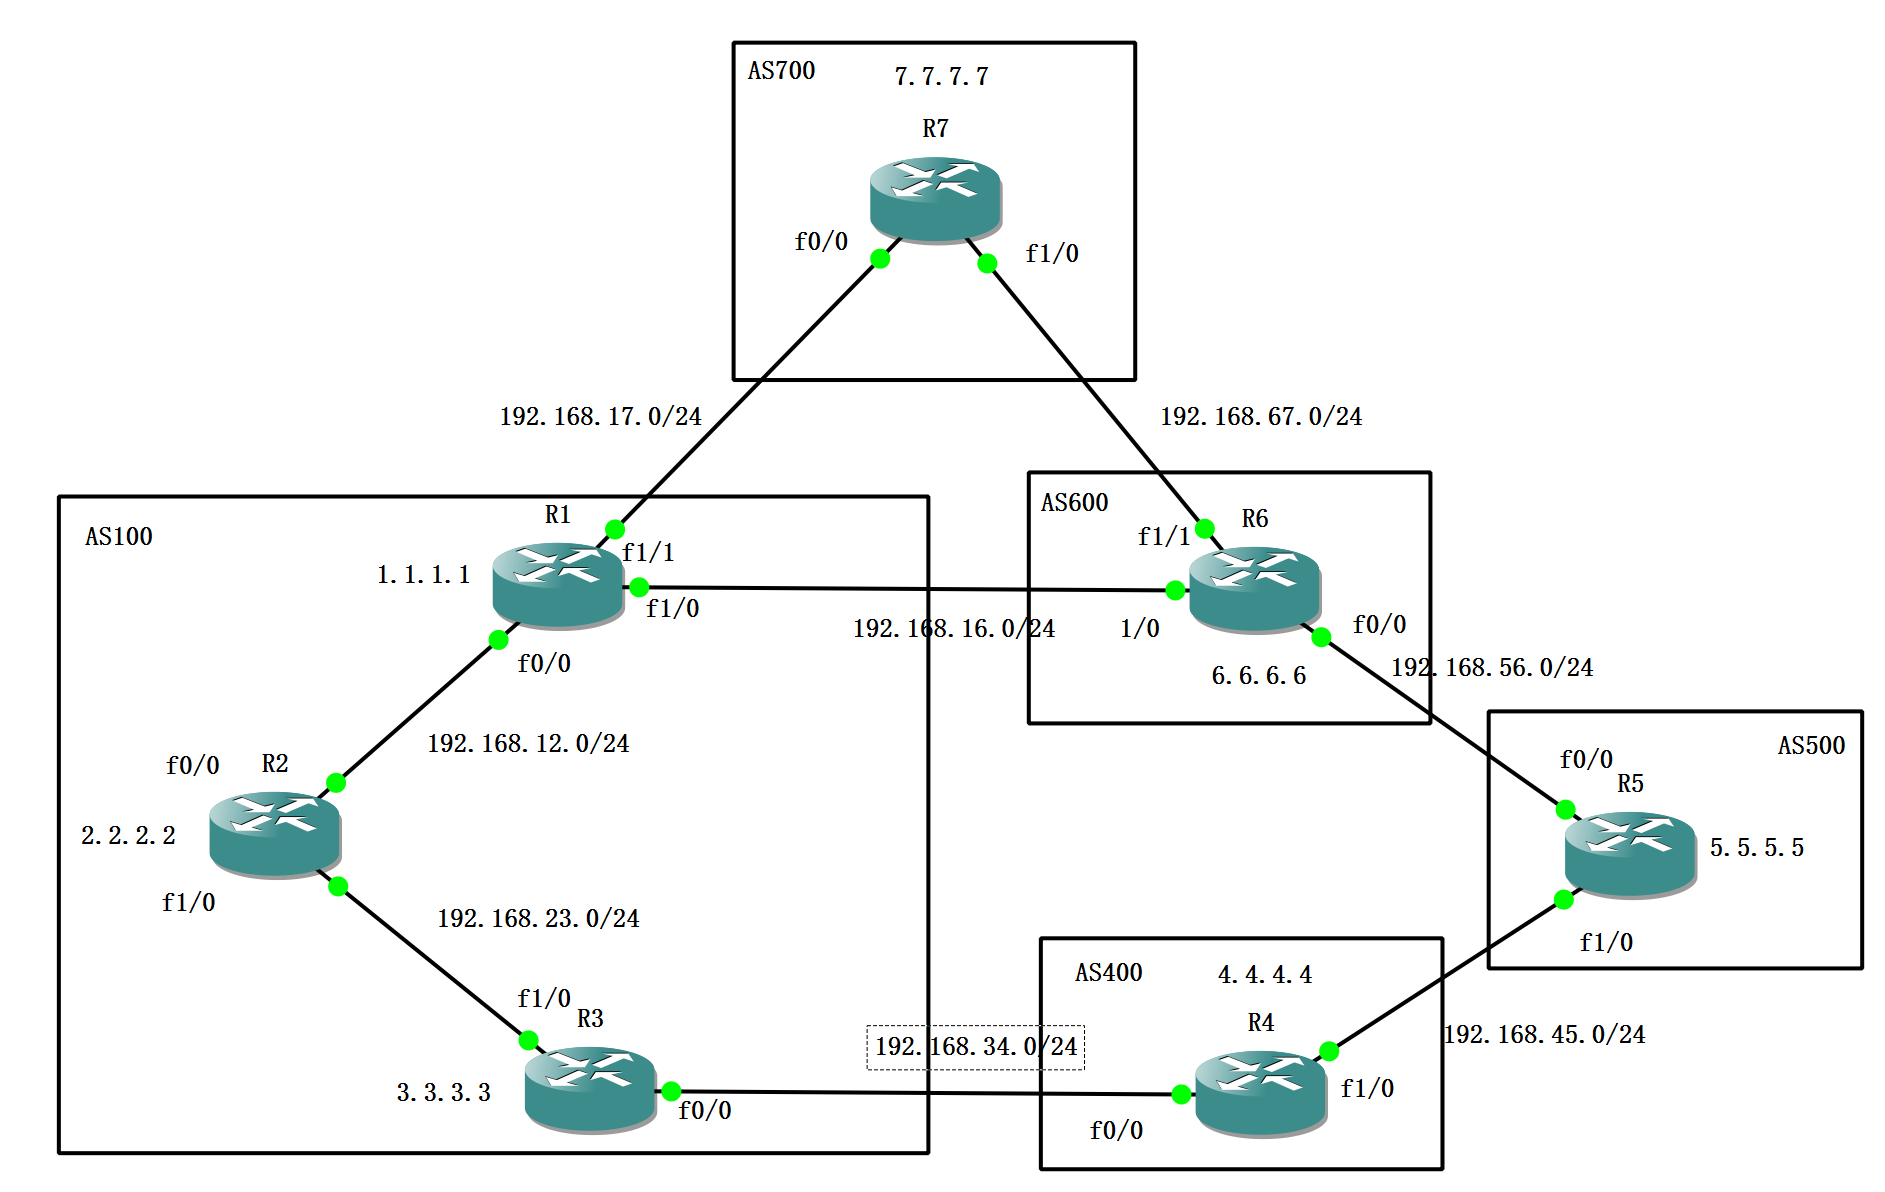
\includegraphics[width=0.8\textwidth,keepaspectratio]{Graph/BGP topology.png}
    \caption{Topology of platform building based on BFD link detection in BGP} 
    \label{fig:Topology of platform building based on BFD link detection in BGP} 
\end{figure}

In AS100, routers R1, R2, and R3 exchange routing information within the 192.168.12.0/24, 192.168.23.0/24, and 192.168.17.0/24 segments, respectively, using the OSPF protocol.R1 is the edge router connected to R7 in AS700. In AS600, router R6 is configured with router R5 in AS500 across the 192.168.56.0/24 segment via the BGP protocol.The connection between R4 in AS400 and R5 in AS500 is not specified.

The inter-AS connection between two border routers in different AS systems is established using the BGP protocol, which facilitates the exchange of routing information between two different ASes and acts as a unique link between them (except for the connection between A1, A6 and A7). The BFD protocol will be deployed on this BGP connection to monitor the difference in behavior between traditional BGP retransmissions and BGP retransmissions with BFD enabled.

Due to the large number of routers involved, this chapter focuses only on router R2, and its subsequent tests and results are also specific to this router. As shown in the Figure \ref{fig:BGProute}, among the BGP routes, for router R2 I used \textcolor{blue}{\textit{neighbor 3.3.3.3 weight 65535}} to amplify the weight of the path to router R3, aiming to select this path as the main path for routing. Then, when R2 wants to access other segments or routers on the segment, the default path is through R3, as shown in the Figure \ref{fig:IProute}. For R2, R1 is its backup route to access other network segments, and the main routes and information pass through R3. When R3 is shutdown, the backup route can be activated to ensure network connectivity.

\begin{figure}[h]
    \centering
    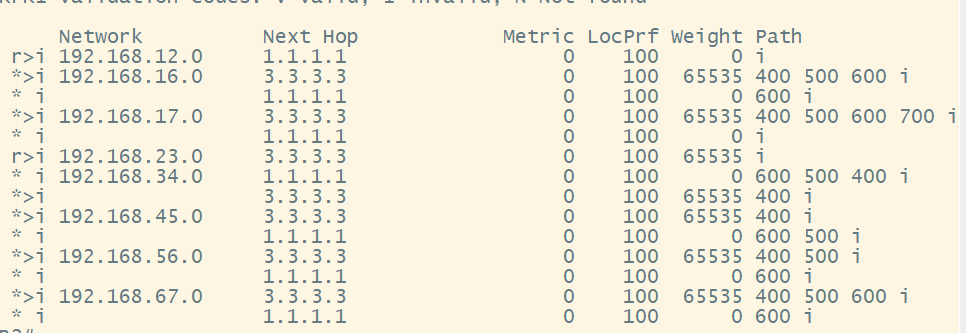
\includegraphics[width=0.8\textwidth,keepaspectratio]{Graph/BGProute.png}
    \caption{BGP route table of R2} 
    \label{fig:BGProute} 
\end{figure}

\begin{figure}[h]
    \centering
    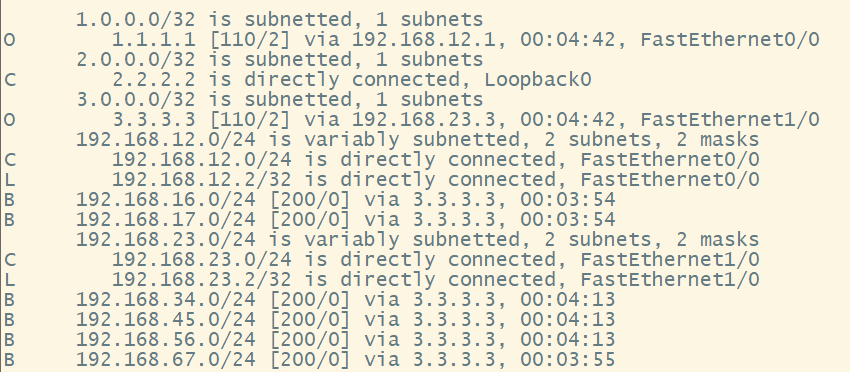
\includegraphics[width=0.8\textwidth,keepaspectratio]{Graph/IProute.png}
    \caption{IP route table of R2} 
    \label{fig:IProute} 
\end{figure}

Trying to access 192.168.17.7, using \textcolor{blue}{\textit{traceroute 192.168.17.7}}, the result is shown in Figure \ref{fig:Traceroute test each hops}.

\begin{figure}[h]
    \centering
    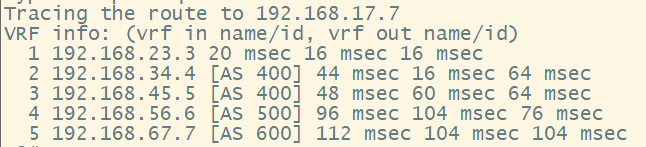
\includegraphics[width=0.7\textwidth,keepaspectratio]{Graph/traceroute.png}
    \caption{Traceroute test each hops} 
    \label{fig:Traceroute test each hops} 
\end{figure}

\subsection{Test and result}
The test environment and test tools are the same as in the previous chapter and will not be repeated here.

The tests in this section focus on the difference in convergence time between deploying BFD with or without  after a BGP peer shutdown. The control group for the test did not apply BFD and used the BGPKEEPLIVE mechanism, while the experimental group enabled the BFD protocol between the R3 and R4 segments. This is accomplished by first making all configurations and segments operational and recording the corresponding timestamps. Then shutdown R4, and observe and record the time when R3 sends the BGP NOTIFICATION packet and R2 redeploys the correct ip route (i.e., all messages go through R1 instead of R3).

First I experimented with the effect of interval time on BGP convergence delay under BFD configuration. The convergence time increases when the BGP system deploys the BFD feature. Where the minimum convergence delay is when 50 ms BFD is applied\cite{ref2}. Since 50ms response is too fast, so in this test I used 100ms, 200ms and 500ms BFD interval time. The test result is shown in Figure \ref{fig:BFD convergence delay}. It is not difficult to conclude that even if the BFD interval time is set to 500ms, the time it takes to respond to a BGP peer interrupt is only about 1400ms. This low latency is sufficient for both small and large networks.

\begin{figure}[h]
    \centering
    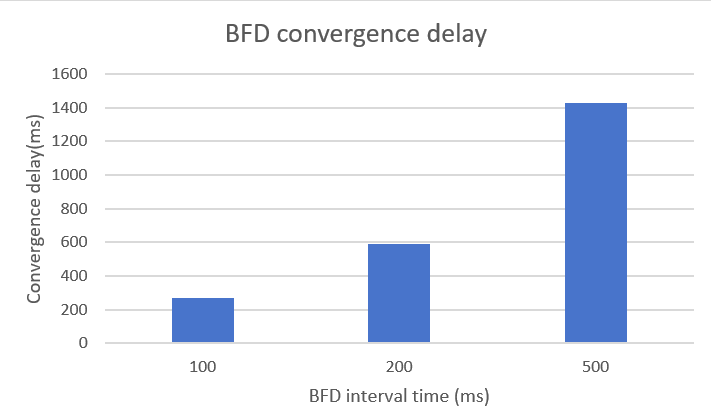
\includegraphics[width=0.7\textwidth,keepaspectratio]{Graph/BFD convergence delay.png}
    \caption{BFD convergence delay} 
    \label{fig:BFD convergence delay} 
\end{figure}

Immediately after that I did three sets of control tests to analyze the differences between the BGP KEEPLIVE mechanism and the BFD protocol by observing the BGP convergence time as Figure \ref{fig:Convergence delay between BGP KEEPALIVE and BFD}.As can be seen by the two comparative bar graphs, the BFD protocol increases the performance of the detection of link failure latency, which will be in the milliseconds range, instead of the seconds of keepalive message detection. This also demonstrates the reliability of the BFD protocol. When in a large BGP network, the convergence time after a router reboot is very long, to achieve BGP fast failure detection, it is necessary to enable the BFD protocol in the BGP alias routers that need to be observed.

\begin{figure}[h]
    \centering
    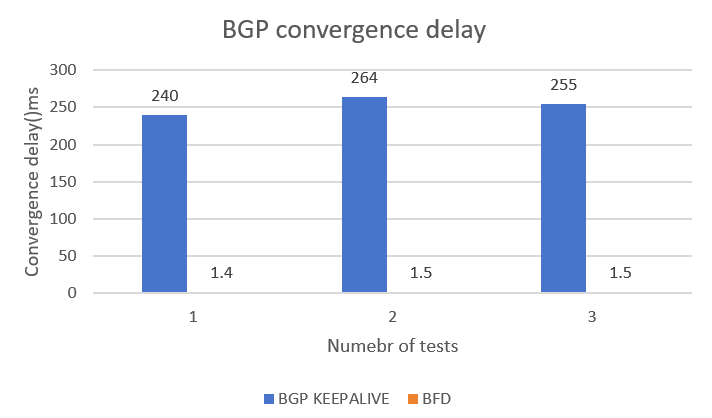
\includegraphics[width=0.7\textwidth,keepaspectratio]{Graph/BGP vs BFD.png}
    \caption{Convergence delay between BGP KEEPALIVE and BFD} 
    \label{fig:Convergence delay between BGP KEEPALIVE and BFD} 
\end{figure}

Finally, to re-observe the ip route of R2, you can also find that it has switched all the routes to pass through the standby router R1, as shown in the Figure \ref{fig:New IP route table of R}. This also proves that BGP routing protocols deployed with BFD can generate the correct routing paths very accurately while having very fast route convergence. The speed and accuracy after deploying BFD is very much guaranteed!

\begin{figure}[h]
    \centering
    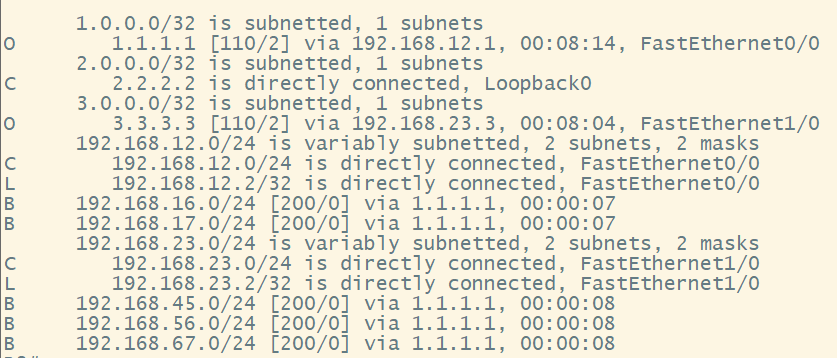
\includegraphics[width=0.7\textwidth,keepaspectratio]{Graph/IP route throught R1.png}
    \caption{New IP route table of R} 
    \label{fig:New IP route table of R2} 
\end{figure}


\newpage
% Section 5
\section{Conclusion and future outlook}
This report extensively examines the integration of the BFD protocol with BGP to enhance fast fault detection within network infrastructures. Through theoretical analyses and practical applications, the report highlights the significant improvements in BFD's responsiveness and reliability of BGP in dynamic network environments. Empirical analyses using GNS3 simulations and real configurations confirm that BFD is effective in reducing fault detection time, thereby optimising network resilience and efficiency. This study paves the way for future research to further optimise and explore the potential of BFD in complex AS environments with the aim of achieving more robust and efficient network operations.

Because of the time constraint and the difficulty of configuration, there are many features in this project that need to be worked on in the future. For example, it is important to implement a more efficient retransmission algorithm for routers in case of BFD configuration to adapt to large-scale networks, and how to configure a network using a combination of BFD and BGP to adapt to the very different underlying architecture of VPP.

I believe that I can gradually learn and improve my knowledge in this area in my future internships, which will also realise the meaning of my independent project.

\newpage
% References
\addcontentsline{toc}{section}{References}
\begin{thebibliography}{99}
    \bibitem{ref1} https://content.cisco.com
    \bibitem{ref2} A. Abaid, M. Hraib, A. B. Ghazzi and S. Sati, "Convergence Time Analysis of Border Gateway Protocol Using GNS3," 2021 IEEE 1st International Maghreb Meeting of the Conference on Sciences and Techniques of Automatic Control and Computer Engineering MI-STA, Tripoli, Libya, 2021, pp. 689-694, doi: 10.1109/MI-STA52233.2021.9464522.
    \bibitem{ref3} https://www.routeprotocol.com/bgp-packet-types/
    \bibitem{ref4} RFC 5880
    \bibitem{ref5} Balyk A, Karpinski M, Naglik A, et al. Using graphic network simulator 3 for DDoS attacks simulation[J]. International Journal of Computing, 2017, 16(4): 219-225.
    \bibitem{ref6} Caesar M, Rexford J. BGP routing policies in ISP networks[J]. IEEE network, 2005, 19(6): 5-11.
    \bibitem{ref7} \begin{CJK}{UTF8}{gbsn} BFD技术白皮书-6W102 \end{CJK}
    \bibitem{ref8} Wang K, Gao L, Lai M. A scalable multithreaded BGP architecture for next generation router[C]//Proceedings of the International Conference on Human-centric Computing 2011 and Embedded and Multimedia Computing 2011: HumanCom \& EMC 2011. Springer Netherlands, 2011: 395-404.
    \bibitem{ref9} Lei G, Mingche L. Fast Failure Recovery Using Multi-threading in BGP[C]//Embedded and Multimedia Computing Technology and Service: EMC 2012. Springer Netherlands, 2012: 163-170.
    \bibitem{ref10} Pallagatti S. Seamless Bidirectional Forwarding Detection (S-BFD) draft-ietf-bfd-seamless-base-03[J]. 2014.
    \bibitem{ref11} Pignataro C, Ward D, Akiya N, et al. Seamless Bidirectional Forwarding Detection (S-BFD)[R]. 2016.
    \bibitem{ref12} Mala S, Mallapur S V. A Brief Analysis of Border Gateway Protocol for Internet Controlling and Malicious Attacks[C]//International Conference on Computing, Communication, Electrical and Biomedical Systems. Cham: Springer International Publishing, 2022: 561-572.
\end{thebibliography}

\newpage

\addcontentsline{toc}{section}{Appendix}
\appendix
\section*{Appendix}
\textbf{Configuration of implementation of chapter 3:}

\noindent AR1:

configure terminal

interface f0/0

ip address 192.168.1.1 255.255.255.0

no shutdown

interface f1/0

ip address 192.168.2.1 255.255.255.0

no shutdown

interface lo0

ip address 1.1.1.1 255.255.255.255


\noindent AR2:

configure terminal

interface f0/0

ip address 192.168.1.2 255.255.255.0

no shutdown

interface f1/0

ip address 10.0.0.1 255.0.0.0

no shutdown

int lo0

ip address 2.2.2.2 255.255.255.255

\noindent APC:

ip 10.0.0.2 255.0.0.0 10.0.0.1

\noindent BR1:

configure terminal

interface f0/0

ip address 192.168.3.1 255.255.255.0

no shutdown

interface f1/0

ip address 192.168.2.2 255.255.255.0

no shutdown

interface lo0

ip address 3.3.3.3 255.255.255.255

\noindent BR2:

configure terminal

interface f0/0

ip address 192.168.3.2 255.255.255.0

no shutdown

interface f1/0

ip address 11.0.0.1 255.0.0.0

no shutdown

interface lo0

ip address 4.4.4.4 255.255.255.255

\noindent BPC:

BPC1> ip 11.0.0.2 255.0.0.0 11.0.0.1

\noindent A area OSPF:

\noindent AR1:

router ospf 100

network 192.168.1.0 0.0.0.255 area 0

network 1.1.1.1 0.0.0.0 area 0

\noindent Ar2:

router ospf 100

network 192.168.1.0 0.0.0.255 area 0

network 10.0.0.0 0.255.255.255 area 0

network 2.2.2.2 0.0.0.0 area 0

\noindent B area RIP:

\noindent BR1:

router rip

network 192.168.3.0

network 3.3.3.3

\noindent BR2:

router rip

network 192.168.3.0

network 11.0.0.0

network 4.4.4.4


\noindent BGP:

\noindent AR1:

conf t

int f0/0

router bgp 100

neighbor 2.2.2.2 remote-as 100

neighbor 2.2.2.2 update-source lo0

neighbor 2.2.2.2 next-hop-self

neighbor 192.168.2.2 remote-as 200

network 10.0.0.0 mask 255.0.0.0

exit

exit

write

\noindent AR2:

conf t

int f0/0

router bgp 100

neighbor 1.1.1.1 remote-as 100

neighbor 1.1.1.1 update-source lo0

exit

exit

write

\noindent BR1:

conf t

int f0/0

router bgp 200

neighbor 4.4.4.4 remote-as 200

neighbor 4.4.4.4 update-source lo0

neighbor 4.4.4.4 next-hop-self

neighbor 192.168.2.1 remote-as 100

network 11.0.0.0 mask 255.0.0.0

exit

exit

write

\noindent BR2:

conf t

int f0/0

router bgp 200

neighbor 3.3.3.3 remote-as 200

neighbor 3.3.3.3 update-source lo0

exit

exit

write


\noindent BFD:

\noindent AR1:

conf t

int f1/0

bfd interval 500 min\_rx 500 multiplier 3

router bgp 100 

neighbor 192.168.2.2 fall-over bfd

exit

exit

\noindent BR1:

conf t

int f1/0

bfd interval 500 min\_rx 500 multiplier 3

router bgp 200 

neighbor 192.168.2.1 fall-over bfd

exit

exit
 
~\\
\noindent \textbf{Configuration of implementation of chapter 4:}

\noindent R1:

configure terminal

interface f0/0

ip address 192.168.12.1 255.255.255.0

no shutdown

interface f1/0

ip address 192.168.16.1 255.255.255.0

no shutdown

interface f1/1

ip address 192.168.17.1 255.255.255.0

no shutdown

interface lo0

ip address 1.1.1.1 255.255.255.255

router ospf 100

network 192.168.12.0 0.0.0.255 area 0

network 1.1.1.1 0.0.0.0 area 0

router bgp 100

neighbor 2.2.2.2 remote-as 100

neighbor 2.2.2.2 update-source lo0

neighbor 2.2.2.2 next-hop-self

neighbor 192.168.16.6 remote-as 600

neighbor 192.168.17.7 remote-as 700

network 192.168.12.0 mask 255.255.255.0

network 192.168.17.0 mask 255.255.255.0

exit

exit


\noindent R2:

configure terminal

interface f0/0

ip address 192.168.12.2 255.255.255.0

no shutdown

interface f1/0

ip address 192.168.23.2 255.255.255.0

no shutdown

interface lo0

ip address 2.2.2.2 255.255.255.255

router ospf 100

network 192.168.12.0 0.0.0.255 area 0

network 192.168.23.0 0.0.0.255 area 0

network 2.2.2.2 0.0.0.0 area 0

router bgp 100

neighbor 1.1.1.1 remote-as 100

neighbor 1.1.1.1 update-source lo0

neighbor 3.3.3.3 remote-as 100

neighbor 3.3.3.3 update-source lo0

exit

exit

\noindent R3:

configure terminal

interface f0/0

ip address 192.168.34.3 255.255.255.0

no shutdown

interface f1/0

ip address 192.168.23.3 255.255.255.0

no shutdown

interface lo0

ip address 3.3.3.3 255.255.255.255

router ospf 100

network 192.168.23.0 0.0.0.255 area 0

network 3.3.3.3 0.0.0.0 area 0

router bgp 100

neighbor 2.2.2.2 remote-as 100

neighbor 2.2.2.2 update-source lo0

neighbor 2.2.2.2 next-hop-self

neighbor 192.168.34.4 remote-as 400

network 192.168.23.0 mask 255.255.255.0

exit

exit

\noindent R4:

configure terminal

interface f0/0

ip address 192.168.34.4 255.255.255.0

no shutdown

interface f1/0

ip address 192.168.45.4 255.255.255.0

no shutdown

interface lo0

ip address 4.4.4.4 255.255.255.255

router bgp 400

neighbor 192.168.34.3 remote-as 100

neighbor 192.168.45.5 remote-as 500

network 192.168.34.0 mask 255.255.255.0

network 192.168.45.0 mask 255.255.255.0

exit

exit

\noindent R5:

configure terminal

interface f0/0

ip address 192.168.56.5 255.255.255.0

no shutdown

interface f1/0

ip address 192.168.45.5 255.255.255.0

no shutdown

interface lo0

ip address 5.5.5.5 255.255.255.255

router bgp 500

neighbor 192.168.45.4 remote-as 400

neighbor 192.168.56.6 remote-as 600

network 192.168.45.0 mask 255.255.255.0

network 192.168.56.0 mask 255.255.255.0

exit

exit

\noindent R6:

configure terminal

interface f0/0

ip address 192.168.56.6 255.255.255.0

no shutdown

interface f1/0

ip address 192.168.16.6 255.255.255.0

no shutdown

interface f1/1

ip address 192.168.67.6 255.255.255.0

no shutdown

interface lo0

ip address 6.6.6.6 255.255.255.255

router bgp 600

neighbor 192.168.16.1 remote-as 100

neighbor 192.168.56.5 remote-as 500

neighbor 192.168.67.7 remote-as 700

network 192.168.16.0 mask 255.255.255.0

network 192.168.56.0 mask 255.255.255.0

network 192.168.67.0 mask 255.255.255.0

exit

exit

\noindent R7:

configure terminal

interface f0/0

ip address 192.168.17.7 255.255.255.0

no shutdown

interface f1/0

ip address 192.168.67.7 255.255.255.0

no shutdown

interface lo0

ip address 7.7.7.7 255.255.255.255

router bgp 700

neighbor 192.168.17.1 remote-as 100

neighbor 192.168.67.6 remote-as 600

network 192.168.17.0 mask 255.255.255.0

network 192.168.67.0 mask 255.255.255.0

exit

exit

~\\
\noindent \textbf {Optinal:(For changing the weight of the path and implement BFD)}

conf t

route-map SET\_LOCAL\_PREF permit 10

set local-preference 200

router bgp 200

neighbor 3.3.3.3 weight 65535

router bgp 100

neighbor 3.3.3.3 route-map SET\_LOCAL\_PREF in

\noindent R3:

conf t

int f0/0

bfd interval 500 min\_rx 500 multiplier 3

router bgp 100 

neighbor 192.168.34.4 fall-over bfd

exit

exit

\noindent Shutdown the router:
conf t

int f0/0

bfd interval 500 min\_rx 500 multiplier 3

router bgp 400 

neighbor 192.168.34.3 fall-over bfd

exit

exit






\end{document}
